\documentclass[xcolor=dvipsnames]{beamer}

\mode<presentation>
% these codes for chinese characters input, if you meet problems with these codes, you can feel free to comment them, or you can try to change your build method to "xelatex"
% \documentclass[xcolor=dvipsnames]{beamer}
% \usepackage{xeCJK}
\usepackage{verbatim}
\usepackage{subfigure} 
\RequirePackage{color}
% For convenience, some of the topics are listed here for users to use.

% \usetheme{AnnArbor}
%\usetheme{Antibes}
%\usetheme{Bergen}
% \usetheme{Berkeley}
%\usetheme{Berlin}
%\usetheme{Boadilla}
% \usetheme{boxes}
% \usetheme{CambridgeUS}
%\usetheme{Copenhagen}
%\usetheme{Darmstadt}
% \usetheme{default}
%\usetheme{Frankfurt}
%\usetheme{Goettingen}
%\usetheme{Hannover}
% \usetheme{Ilmenau}
% \usetheme{JuanLesPins}
%  \usetheme{Luebeck}
 \usetheme{Madrid}
% \usetheme{Malmoe}
%\usetheme{Marburg}
% \usetheme{Montpellier}
% \usetheme{PaloAlto}
% \usetheme{Pittsburgh}
% \usetheme{Rochester}
% \usetheme{Singapore}
% \usetheme{Szeged}
% \usetheme{Warsaw}

\definecolor{sjtu-red}{RGB}{184,45,40} 
\definecolor{sjtu-white}{RGB}{255,255,255}
\definecolor{sjtu-blue}{RGB}{21,65,146}
\definecolor{sjtu-black}{RGB}{0,0,0}

% Uncomment the following code to get the color gradient on the slide (Decaying from sjtu-red to sjtu-white).


% \useoutertheme{shadow}
% \usepackage{tikz}
% \usetikzlibrary{shadings}
% \colorlet{titleleft}{sjtu-red}
% \colorlet{titleright}{sjtu-red!45!sjtu-white}
% \makeatletter
% \pgfdeclarehorizontalshading[titleleft,titleright]{beamer@frametitleshade}{\paperheight}{%
%   color(0pt)=(titleleft);
%   color(\paperwidth)=(titleright)}
% \makeatother

% End of gradient slide title effect.

\setbeamercolor{section in head/foot}{bg=sjtu-blue, fg=sjtu-white}
\setbeamercolor{subsection in head/foot}{bg=sjtu-blue, fg=sjtu-white}
\setbeamercolor{frametitle}{bg=sjtu-blue, fg=sjtu-white}
\setbeamercolor{title}{bg=sjtu-blue, fg=sjtu-white}
\setbeamercolor{alerted text}{fg=sjtu-blue}
\setbeamercolor{block title}{fg=sjtu-white}
\setbeamercolor{block body}{fg=sjtu-black}

\setbeamertemplate{theorems}[numbered]
\setbeamertemplate{propositions}[numbered]

\setbeamertemplate{bibliography item}{\insertbiblabel}

\setbeamertemplate{title page}[default][colsep=-4bp,rounded=true, shadow=true]

\title[Online FAST]{Online-FAST: An Online Fairness Assured Service Recommendation Strategy Considering Service Capacity Constraints}

\subtitle{2020 Fall CS222 Group Project Presentation}

% You can uncommit one of this code block to change
% from one-author's mode to muli-author's mode which is 
% displayed in the title page.
% \author{Authors' name}
% \institute[Shanghai Jiao Tong University] % (optional, but mostly needed)
% {
%   School of Electronic Information and Electrical Engineering\\
%   Shanghai Jiao Tong University
% }

\author[L. Zhou, H. Yang, S. Dong] {Litao Zhou, Hongbo Yang, Shiwen Dong}

\institute[SJTU-IEEE] % (optional)
{
  IEEE Class F1803016 \\
  School of Electronic Information and Electrical Engineering\\
  Shanghai Jiao Tong University
}

\titlegraphic{
  % Uncomment the other code line below to change the logo from English version to Chinese.  
   % 
\includegraphics[width=4.4cm]{sjtu-logo}
   
\includegraphics[width=4cm]{img/sjtu-logo-en.png}
}

\date{\today}

% Uncomment this, if you want the table of contents to pop up at the beginning of each subsection:

% End of the table-content part
% \AtBeginSection[]
% {
%   \begin{frame}{Outline}
%       \tableofcontents[currentsection,currentsubsection,hideothersubsections]
%   \end{frame}
% }
\begin{document}

\begin{frame}
  \titlepage
\end{frame}

\logo{
\includegraphics[height=1cm]{img/sjtu.png}}

% \begin{frame}{Outline}
%   \tableofcontents[hideallsubsections]
% \end{frame}

\section{Background}

\begin{frame}{Background}% {Optional Subtitle}
\begin{block}{Recommendation Fairness}
Consider a service recommendation scenario with capacity constraints, 
some customers may not able to get satisfactory service quality.
%%%
\end{block}

% zlt add description here
\begin{figure}[H]
  \centering
  \subfigure[Shared Bike Recommendation (A previous project at EI333)]{
    \begin{minipage}[t]{0.4\linewidth}
    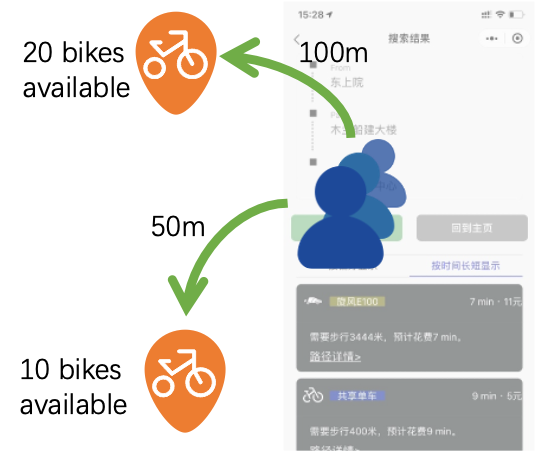
\includegraphics[width=0.9\textwidth]{img/intro_case1.png}
    \end{minipage}
  }
  \hspace{0.2in}
  \subfigure[Restaurant Recommendation]{
    \begin{minipage}[t]{0.4\linewidth}
    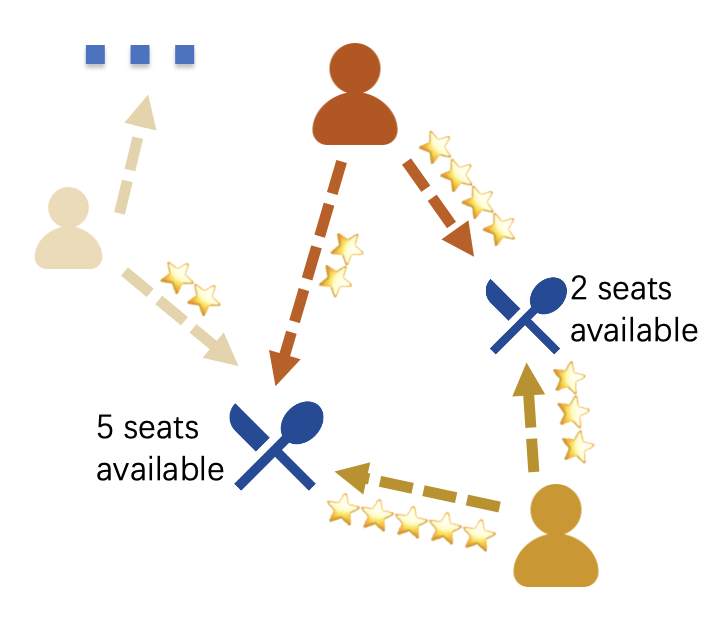
\includegraphics[width=0.9\textwidth]{img/intro_case2.png}
    \end{minipage}
  }
\end{figure}

We need to (1) meet the capacity constraint, (2) ensure individual fairness, (3) maintain recommendation quality.

\end{frame}







\begin{frame}{Background\footnote{Yao Wu, \textbf{Jian Cao}, and Guandong Xu. “FAST: A Fairness Assured Service Recommendation StrategyConsidering Service Capacity Constraint”. In: Service-Oriented Computing, (ICSOC 2020)}}

\begin{block}{FAST: Fairness Assured Service Recommendation Strategy}
\textbf{Significance}
  \begin{enumerate}
      \item Establishing a metric for fairness;
      \item Giving an algorithm to adjust recommendation results to ensure Fairness among users in N rounds while maintaining a high recommendation quality
  \end{enumerate}


 \textbf{Shortcoming}
 \begin{enumerate}
     \item High computational complexity with at least a computation of
$O(n log n)$ per request;
     \item The proposed algorithm can only calculate a global recommendation plan
after all users’ information has been gathered
     
 \end{enumerate}
\end{block}

    
\end{frame}






\begin{frame}{Background}

 \begin{block}{Shortcoming of FAST}
  \begin{enumerate}
     \item High computational complexity with at least a computation of $O(n log n)$ per request;
     \item The proposed algorithm can only calculate a global recommendation plan after all users’ information has been gathered
     \item The analysis of FAST assumes a \textbf{fixed} user set.
     
 \end{enumerate}
 \end{block}


~\\

These Shortcomings hinder FAST from online deployment.
~\\

Our Goal: Establish an Online FAST algorithm.
     \begin{enumerate}
     \item Lower its computing complexity
     \item Give a recommended service whenever it gets a request
     \item Allow users come with a probability
     
 \end{enumerate}
\end{frame}



% show 我们用的概念的定义
\begin{frame}{Terminologies}% {Optional Subtitle}

\begin{figure}
    \centering
    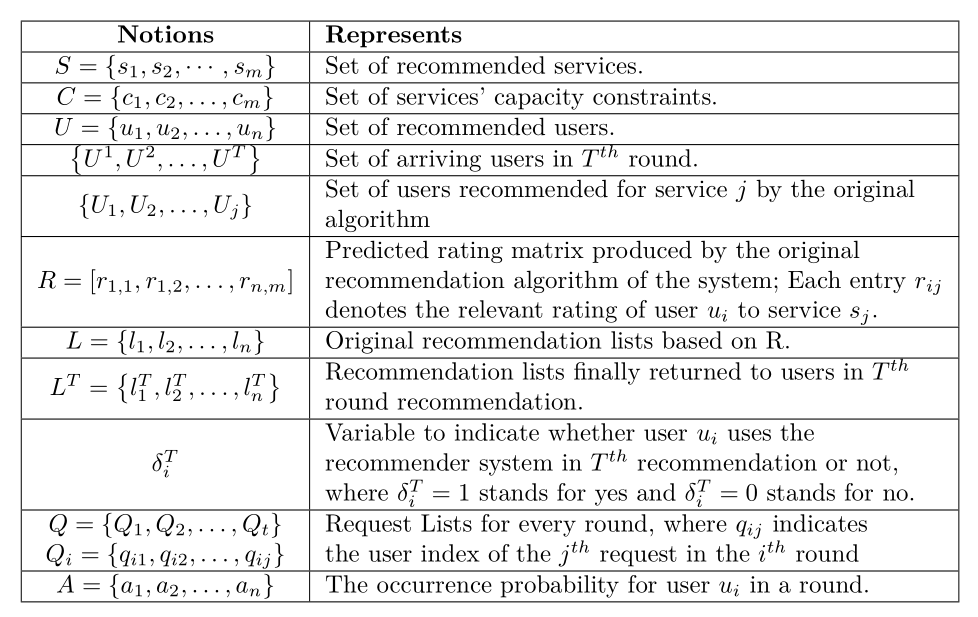
\includegraphics[width=0.9\textwidth]{img/notion.png}
    \caption{Basic Notions}
    \label{notion}
\end{figure}
   
\end{frame}

%%%%%%%%%

\begin{frame}{Definition}% {Optional Subtitle}
\begin{block}{Definition 1: Ideal Probability}
\begin{equation}
p_{j}^{T}=\frac{\sum_{u_{i} \in U_{j}} \sum_{t=0}^{T} \delta_{i}^{t} \cdot  \operatorname{Is\_In}\left(s_{j}, l_{i}^{t}, N\right)}{\sum_{u_{i} \in U_{j}} \sum_{t=0}^{T} \delta_{i}^{t}}
\end{equation}
\end{block}
% question: sum to average or average to sum when counting probability
\begin{block}{Definition 2: Actual Probability} 
\begin{equation}
p_{i, j}^{T}=\frac{\sum_{t=0}^{T} \delta_{i}^{t} \cdot \operatorname{Is\_In}\left(s_{j}, l_{i}^{t}, N\right)}{\sum_{t=0}^{T} \delta_{i}^{t}}
\end{equation}
where $\delta_{i}^{t}$ indicates the possibility that user $i$ is the owner of a request in the $t^{\text{th}}$ round.
\end{block}
where
\begin{equation}\operatorname{Is\_In}\left(s_{j}, l i s t, N\right)=\left\{\begin{array}{l}0 \text { if } s_{j} \text { is not in the top } N \text { sub-list of list } \\ 1 \text { if } s_{j} \text { is in the top } N \text { sub-list of list }\end{array}\right.\end{equation}
\end{frame}

\begin{frame}{Definition}% {Optional Subtitle}

\begin{block}{Definition 3: Service Fairness Degree}
  Fairness degree of user $u_{i}$ on service $s_{j}$ up to $T^{t h}$ round recommendation:
\begin{equation}
F_{i, j}^{T}=\frac{p_{i, j}^{T}-p_{j}^{T}}{p_{j}^{T}}
\label{eqn:def_fairness}
\end{equation}

\end{block}
This definition gives a metric for fairness. The larger $|F|$ is,
the less fairness the recommendation has.

And we can define the Service Fairness Degree among the Top-N list of one user.

\begin{block}{Definition 4: Top-N Overall Fairness Degree}
  Overall fairness degree of user $u_{i}$ up to $T^{t h}$ round recommendation:
\begin{equation}
F_{i}^{T}=\sum_{s_{j} \in l(N)_{i}} F_{i, j}^{T}
\end{equation}

\end{block}
\end{frame}


\begin{frame}{Recommendation Quality Metric}% {Optional Subtitle}

\begin{block}{Definition 5:  Recommendation Quality Metric}
 Quality of outputted recommendation list $l_{i}^{T}$ of user $u_{i}$ on $T^{\text {th }}$ round recommendation:
\begin{equation}
    q_{i}^{T}=\frac{\sum_{s_{j} \in l(N)_{i} \cap l(N)_{i}^{t}} \frac{r_{i, j}}{\log _{2}\left(p_{i, j}^{T}+1\right)}}{r_{i, l(N)_{i}[0]}}
\end{equation}
where $l(N)_{i}[0]$ represents the subscript index of the service appearing at the top position of $l(N)_{i},$ and $p_{i, j}^{T}$ is the position of service $s_{j}$ in $l(N)_{i}$
\end{block}

\begin{enumerate}
    \item Considering the quality of $l(N)_{i}$, namely the top-N list;
    \item Normalizing the quality score with the highest rating of $l(N)_{i}$ as the denominator.
\end{enumerate}

 

\end{frame}


\section{Problem Formulation}

Based on the previous metrics, we can get the formal definition of fairness assured online recommendation problem for services with capacity constraints.

\begin{definition}[Fairness Assured Recommendation Online Problem for Services with Capacity Constraints.]

\textbf{Given}, Relevance rating matrix $R$ and original recommendation lists $\{L\}$ generated by a conventional recommendation algorithm, the set of services' capacity constraint $C$, a positive integer $N$, an set of ordered lists of recommendation requests $Q$ where $q_{ij}$ is from a set of users $U$, indicating the $j^{\text{th}}$ request in $i^{\text{th}}$ round. 


\textbf{Objective}, Finding a top-$N$ recommendation list for each request to minimize $D(F_i^T)$, where $D\left(F_{i}^{T}\right)$ represents the variance among Top-N Fairness of all users.

\textbf{Constraint},
\begin{enumerate}\setlength{\itemsep}{-0.1cm}
    \item Capacity: keeping $\forall c_{j} \in C, c_{j} \geqslant \sum_{u_{i} \in U} \delta_{i}^{T} \cdot  \operatorname{Is\_In}\left(s_{j}, l_{i}^{T}, N\right)$
    \item Recommendation Quality: preserving $\sum_{u_{i} \in U} q_{i}^{T}$ at a high level
    \item Online Property: The recommendation for $q_{ij}$ should not be affected by $q_{i'j'}$ where $ i' > i$ or  $j'> j \And i' = i$ .
\end{enumerate}

\end{definition}

The improvement in our formulation compared with the original FAST system is that our problem regulates that the requests should be taken sequentially. Our problem also takes a user coming probability $A$ instead of the fixed user set as input. These two differences are what we believe to be of the greatest help for online implementation.


% 我们提出的算法(pseudo code)
% \begin{frame}{Offline-FAST}
% Former work towards fairness:

% \begin{figure}
%     \centering
%     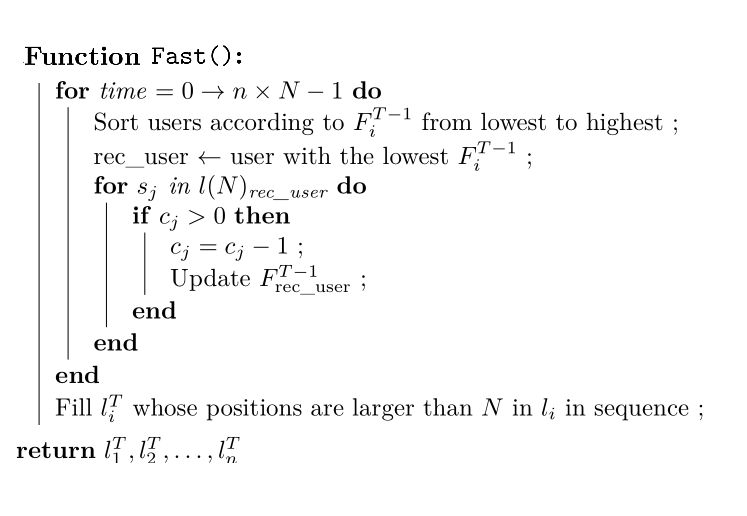
\includegraphics[width=1\textwidth]{img/a1.png}
%     \label{Algo1}
% \end{figure}
% \begin{figure}
%     \centering
%     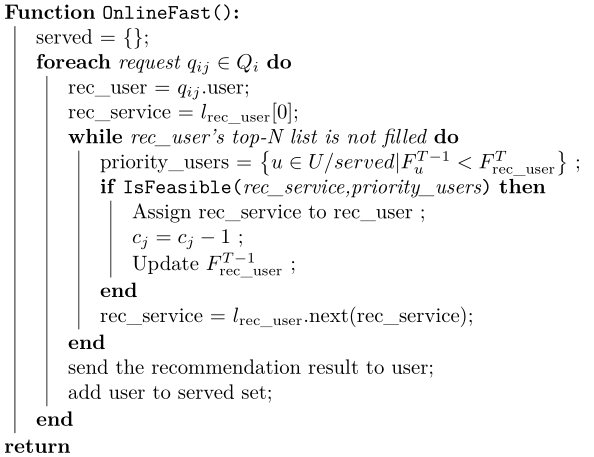
\includegraphics[width=0.8\textwidth]{img/a2.png}
%     \label{Algo2}
% \end{figure}
% \end{frame}

\begin{frame}{Online-FAST}
\begin{figure}[H]
  \centering
  \subfigure{
    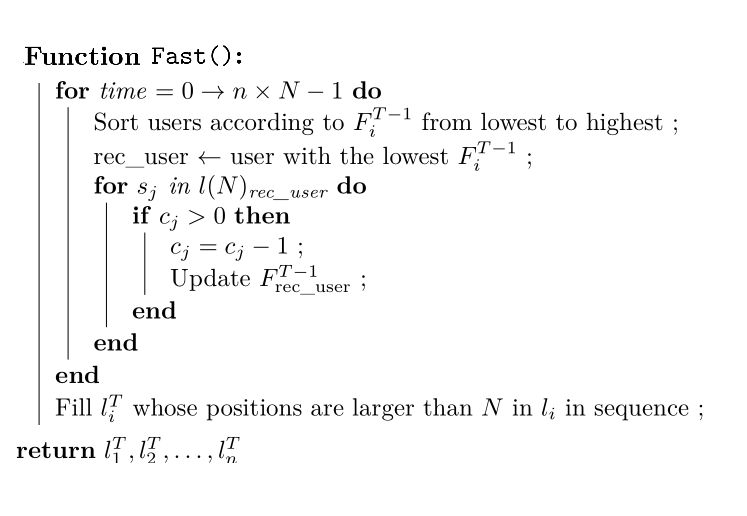
\includegraphics[width=0.45\textwidth]{img/a1.png}}
  \hspace{0.2in} % 两图片之间的距离
  \subfigure{
    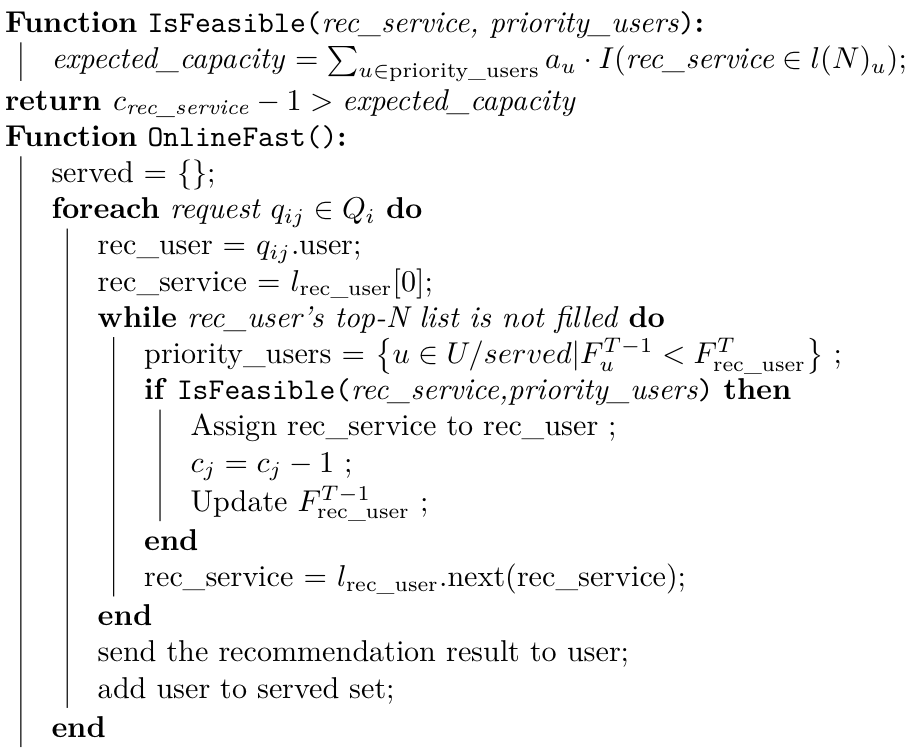
\includegraphics[width=0.45\textwidth]{img/algorithm2_new.png}}
   \caption{Comparing 2 algorithms}
\end{figure}

By using \texttt{IsFeasible} as a heuristic, we avoid the high computational cost of sorting and eliminate the dependency on future requests in Offline-FAST.
 
\end{frame}


% 我们工作的'理论基础'
% 放上定理即可
\begin{frame}{Analysis of Online-FAST}
\begin{block}{Theorem 1: Fairness Degree Converges to Zero}
Given the arriving probability $A$ for the user set, the sum of Top-N Fairness Degree of all the users in each round will approach to zero (i.e.  $\lim_{T \rightarrow \infty}\sum_{u_{i} \in U} F_{i}^{T}=0$) if and only if the users share a same arriving probability.
\label{thm1}
\end{block}
% ps: Proof of Theorem 1 can be checked in our paper.\\


\begin{figure}[H]
  \centering
  \subfigure{
    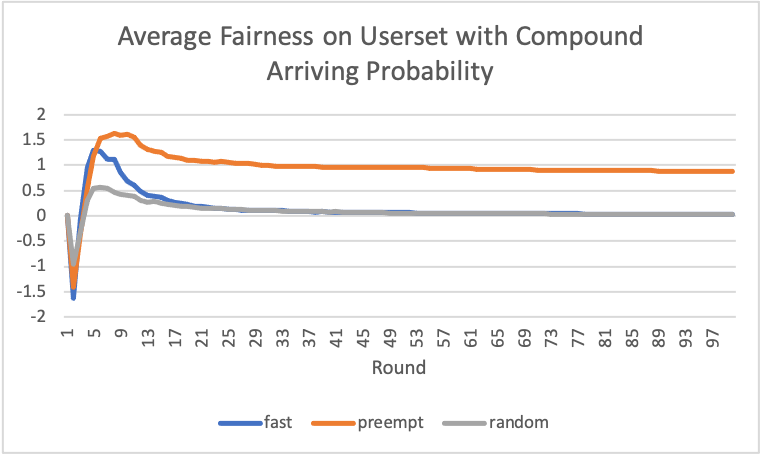
\includegraphics[scale=0.21]{img/thr1.png}}
  \hspace{0.1in} % 两图片之间的距离
  \subfigure{
    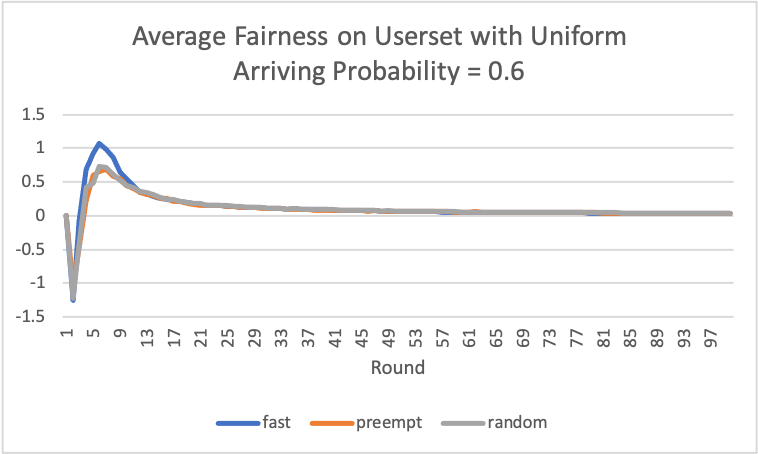
\includegraphics[scale=0.21]{img/thr2.png}}
  \caption{An intuitive interpretation of Theorem 1}
\end{figure}

\end{frame}

\begin{frame}{Analysis of Online-FAST}
%第二个定理依赖了一些直觉上的推论和随机性的假设
Based on the result of Theorem 1,
we have the following claim:
\begin{block}{Claim: Variance Convergence}
For a group of users with the same arriving probability, assume the arrival of them are uniformly distributed. The variance among the Top-N fairness of them $D\left(F_{i}^{T}\right)$ converges with the recommended round $T$.
\end{block}
\begin{enumerate}
    \item This claim is based on intuitive inference and assumption of randomness;
    \item Its validness and versatility can be checked with experiments in real cases.
\end{enumerate}
\end{frame}




% 我们为验证算法有效性做的实验

% 介绍dataset
% Dataset的生成方式
\begin{frame}{Experiment: Dataset Preparation}
    \begin{block}{Dataset}
    \begin{enumerate}
        \item Yelp Dataset: real world dataset
        \begin{enumerate}
        \item Phoenix
        \item Toronto
        \end{enumerate}
        
        \item Synthetic dataset, generated by different param-settings
        \begin{enumerate}
        \item Dataset 1 : Slack capacity constraints 
        \item Dataset 2 : balanced capacity constraints
        \item Dataset 3 : prominent capacity conflicts 
        \item Dataset 4 : serious capacity conflicts
        \end{enumerate}
        
    \end{enumerate}
    \end{block}
    \begin{block}{Evaluation Metric}

         \begin{enumerate}
        \item Total quality of recommendations of each user
        \item Variance among Top-N Fairness of all users
        \end{enumerate}

    
        \end{block}
    
\end{frame}





% 介绍使用到对比的另两种方法
\begin{frame}{Experiment: Constrast Algorithms}
    We compare our algorithm against the following two baseline methods
    
    \begin{block}{Preempt Strategy}
A kind of first-come first-served (FCFS) process scheduling algorithm which doesn’t take fairness into consideration
    
        \end{block}
        \begin{block}{Random Strategy}
Assign Services to users randomly, which can also assure Top-N Fairness in the long run.
        \end{block}
    
\end{frame}




% 分别介绍真实数据集和人工数据集的实验情况,插入图表
\begin{frame}{Experiment on Yelp Dataset}


\begin{figure}[htbp]
\centering
\subfigure{
\begin{minipage}[t]{0.36\linewidth}
\centering
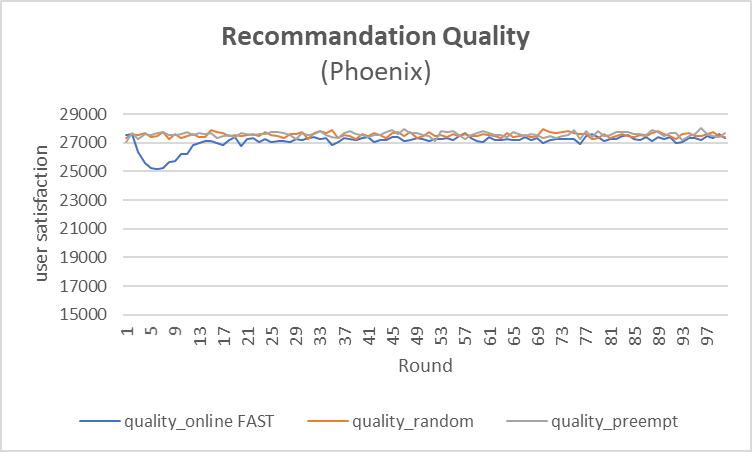
\includegraphics[width=1.6in]{img/2_q_p.png}
\end{minipage}%
}%
\subfigure{
\begin{minipage}[t]{0.36\linewidth}
\centering
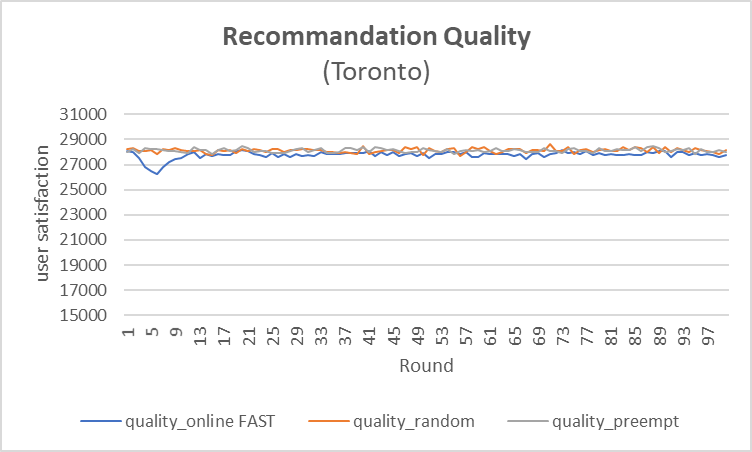
\includegraphics[width=1.6in]{img/2_q_t.png}
\end{minipage}%
}%
\caption{Online FAST keeps Recommendation Quality at a high level}
\end{figure}

\begin{figure}
\subfigure{
\begin{minipage}[t]{0.36\linewidth}
\centering
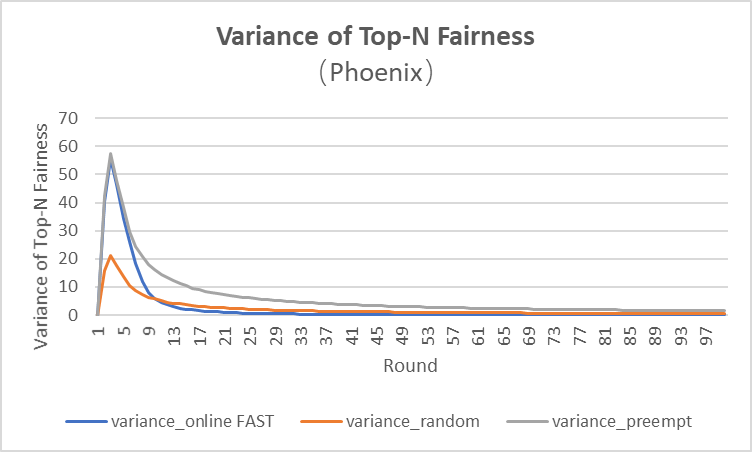
\includegraphics[width=1.6in]{img/2_v_p.png}
\end{minipage}
}%
\subfigure{
\begin{minipage}[t]{0.36\linewidth}
\centering
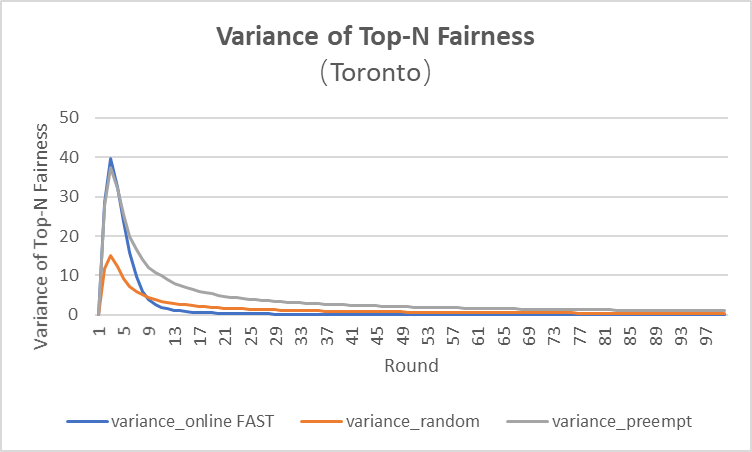
\includegraphics[width=1.6in]{img/2_v_t.png}
\end{minipage}
}%
\centering
\caption{Online FAST shows better convergence property (Arrival Probability = 0.8, N = 5)}
\end{figure}
\end{frame}


\begin{frame}{Experiment on Synthetic Dataset }

\begin{figure}[htbp]
\centering
\subfigure[Dataset 1]{
\begin{minipage}[t]{0.36\linewidth}
\centering
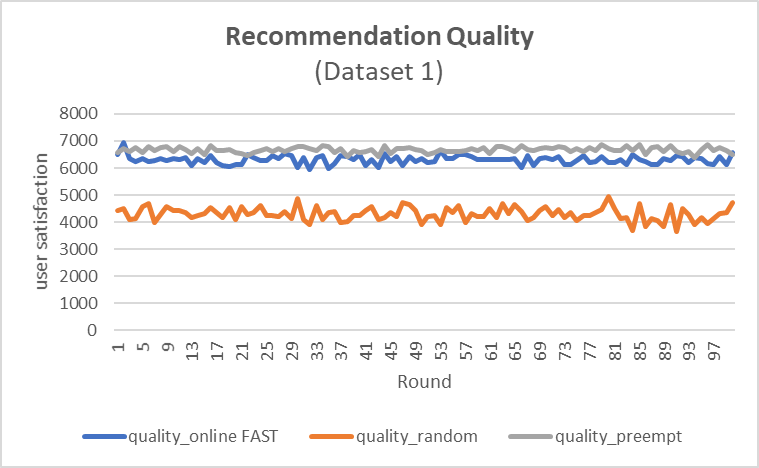
\includegraphics[width=1.6in]{img/1_q_1.png}
\end{minipage}%
}%
\subfigure[Dataset 2]{
\begin{minipage}[t]{0.36\linewidth}
\centering
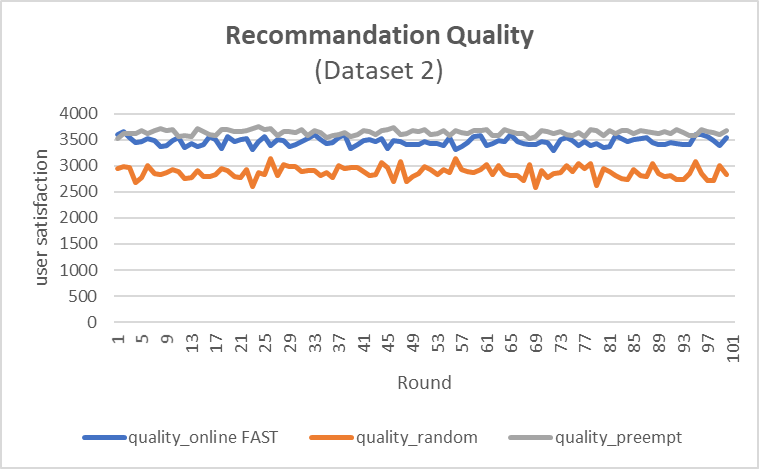
\includegraphics[width=1.6in]{img/1_q_2.png}
\end{minipage}%
}%

\subfigure[ Dataset 3]{
\begin{minipage}[t]{0.36\linewidth}
\centering
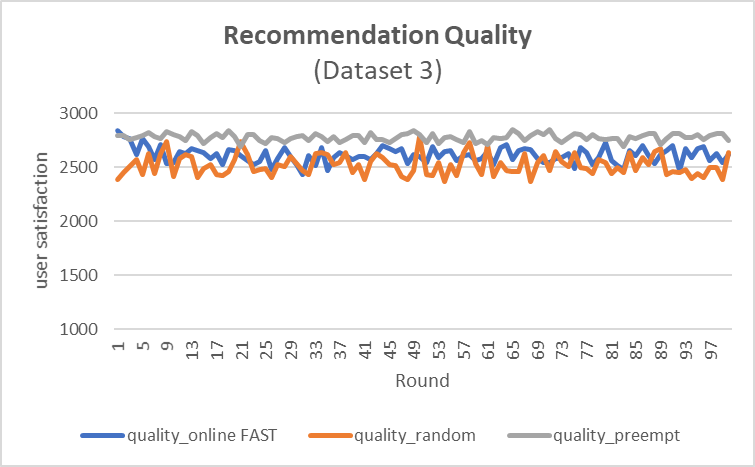
\includegraphics[width=1.6in]{img/1_q_3.png}
\end{minipage}
}%
\subfigure[Dataset 4]{
\begin{minipage}[t]{0.36\linewidth}
\centering
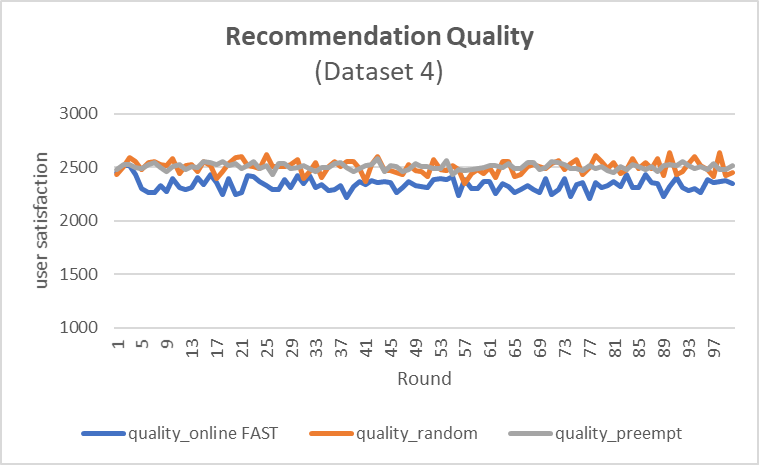
\includegraphics[width=1.6in]{img/1_q_4.png}
\end{minipage}
}%
\centering
\caption{Recommendation Quality of Online-FAST is steady under different levels of capacity constraints\ (Arrival Probability = 0.6, N = 5)}
% \label{fig:RQ}
\end{figure}
\end{frame}


\begin{frame}{Experiment on Synthetic Dataset}

\begin{figure}[htbp]
\centering
\subfigure[Dataset 1]{
\begin{minipage}[t]{0.36\linewidth}
\centering
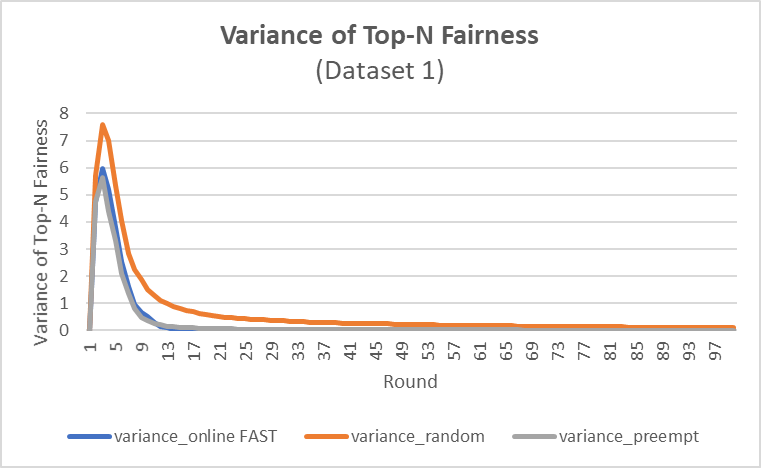
\includegraphics[width=1.6in]{img/1_v_1.png}
\end{minipage}%
}%
\subfigure[Dataset 2]{
\begin{minipage}[t]{0.36\linewidth}
\centering
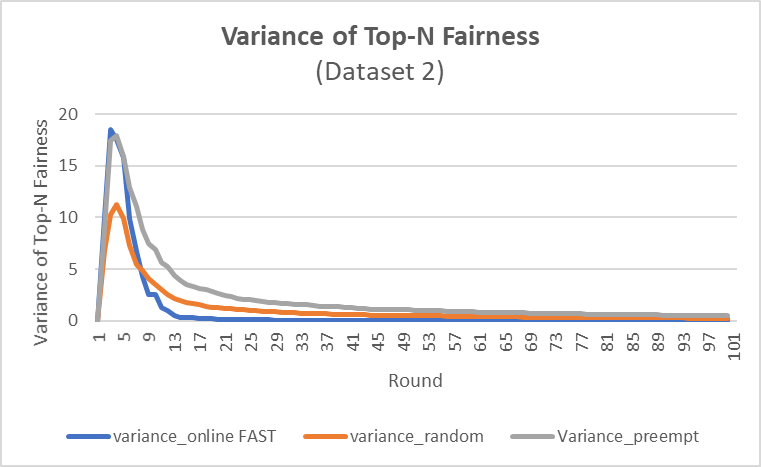
\includegraphics[width=1.6in]{img/1_v_2.png}
\end{minipage}%
}%

\subfigure[ Dataset 3]{
\begin{minipage}[t]{0.36\linewidth}
\centering
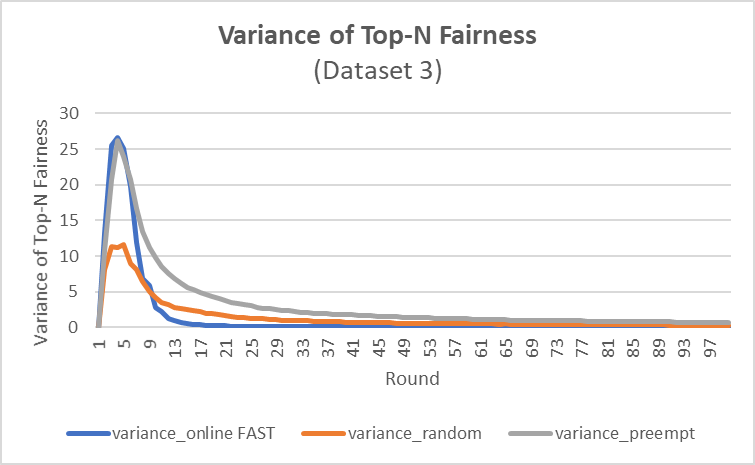
\includegraphics[width=1.6in]{img/1_v_3.png}
\end{minipage}
}%
\subfigure[Dataset 4]{
\begin{minipage}[t]{0.36\linewidth}
\centering
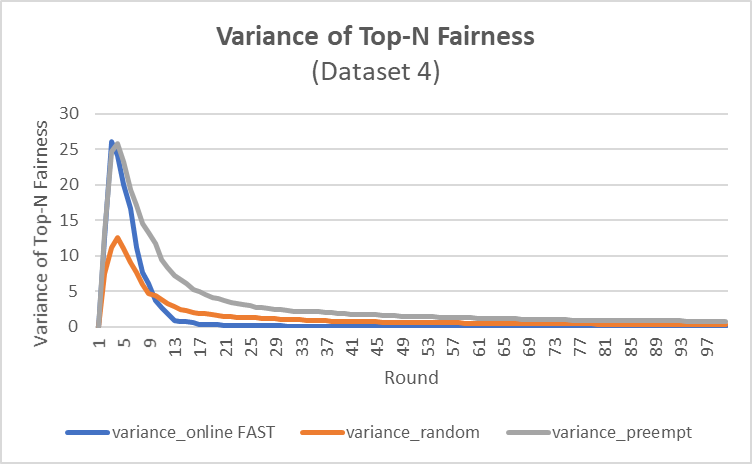
\includegraphics[width=1.6in]{img/1_v_4.png}
\end{minipage}
}%
\centering
\caption{Variance of Top-N Fairness can converge under different levels of capacity constraints (Arrival Probability = 0.6, N = 5)}
\end{figure}
\end{frame}


\begin{frame}{Experiment on Synthetic Dataset}

\begin{figure}[htbp]
\centering
\subfigure[P=0.5]{
\begin{minipage}[t]{0.36\linewidth}
\centering
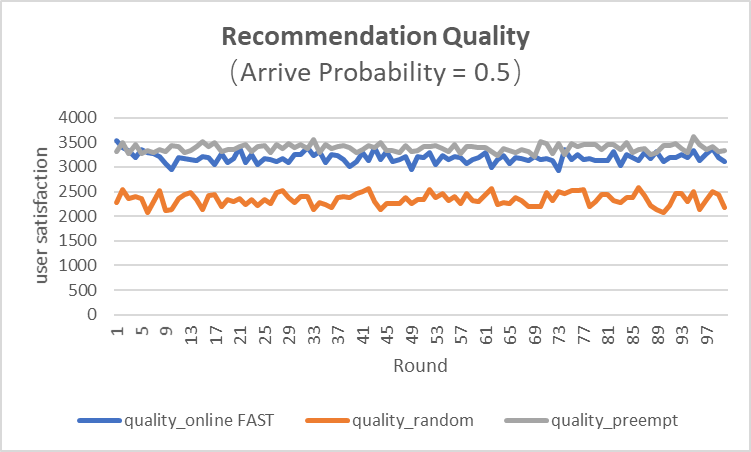
\includegraphics[width=1.6in]{img/3_q_0.5.png}
\end{minipage}%
}%
\subfigure[P=0.6]{
\begin{minipage}[t]{0.36\linewidth}
\centering
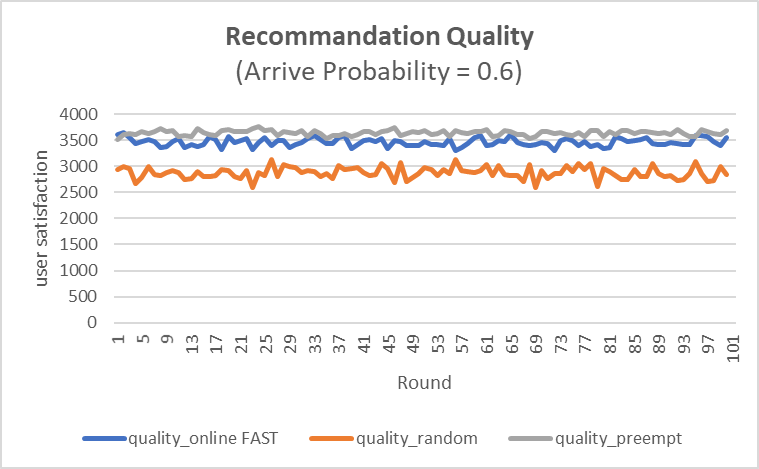
\includegraphics[width=1.6in]{img/3_q_0.6.png}
\end{minipage}%
}%

\subfigure[P=0.7]{
\begin{minipage}[t]{0.36\linewidth}
\centering
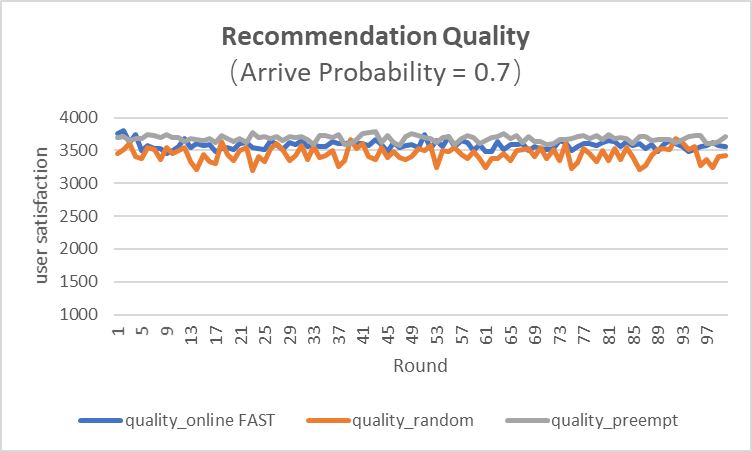
\includegraphics[width=1.6in]{img/3_q_0.7.png}
\end{minipage}
}%
\subfigure[P=0.8]{
\begin{minipage}[t]{0.36\linewidth}
\centering
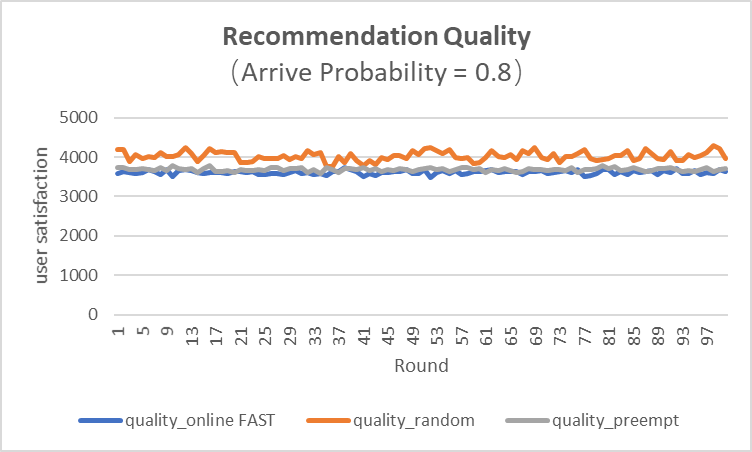
\includegraphics[width=1.6in]{img/3_q_0.8.png}
\end{minipage}
}%
\centering
\caption{Recommendation Quality is steady under different arriving probability  (on Balanced Capacity Constraints Dataset, N = 5)}
\end{figure}
\end{frame}








%%%%%
\begin{frame}{Conclusion}

In this paper, we further expand the concept and application of individual fairness by improving FAST algorithm. To be specific, we first 

\begin{block}{Our Contributions}
\begin{enumerate}
    \item Introduce user sets with arrival probability into the original FAST framework, and formally prove the soundness of fairness degree.
    \item Make the FAST algorithm more suitable for online deployment by designing an online algorithm with
    \begin{itemize}
        \item $O(N)$ cost per request, compared with $O(N \log N)$ in Offline-FAST
        \item Making recommendations independent of future requests
    \end{itemize}
\end{enumerate}
\end{block}

\begin{block}{Future Work}
\begin{enumerate}
    \item Recommendation for users with diverse arriving probability
    \item Dynamic recommendation results per round from the original algorithm
\end{enumerate}
\end{block}
\end{frame}

\input{parts/appendix}

\end{document}